\chapter{ORC System Model Validation, Analysis, and Case Study Results}
\label{ch:analysis}

With the ORC prime power system model constructed as described in \autoref{ch:model}, simulations can be conducted to validate it and verify the model simulates a system as expected. After validation, two case studies, a greenfield and brownfield microgrid, can be investigated and analyzed in order to determine whether geothermal organic Rankine cycle generators can be viably used as primary power sources.

\section{Validation}
%Before simulating  the greenfield and brown field case study scenarios, the model needs to be validated. 
The model validation is conducted by comparing the results of an ORC test with the simulation results under similar conditions. The test, performed in 2013, is from the University of Alaska Fairbanks and is documented in a report by Lin et al. \cite{Lin2014}. The report details the process of testing an Electratherm Green Machine ORC system in a controlled environment at the UAF power plant.
%and in the field for waste heat reclamation of a diesel generator at the Tok, Alaska powerhouse.

During the sizing of the ORC system turbine, $\eta_{turbine}$, and pump, $\eta_{pump}$, efficiencies as well as heat exchanger areas, $A_{evap}$ and $A_{cond}$, and transfer coefficients, $U_{evap}$ and $U_{cond}$, were assumed based off of published values and conventional practice, but final values were not reported. These assumed values are used as the input of the model. All of the non-variable ORC prime power system parameters for the validation can be seen in \autoref{tab:verification_ORC_params}.
\begin{table}%[h]
	\centering
	\caption{Input parameters for the validation of the ORC prime power system model.}
	%\rowcolors{5}{}{gray!10}
	\label{tab:verification_ORC_params}
	\begin{tabular}{rl}
		\toprule
		           Parameter & Value                                        \\ \midrule
		         $U_{evap}$ & 1500 \si{\watt\per\kelvin\per\meter\squared} \\
		         $A_{evap}$ & 26.5 \si{\meter\squared}                     \\
		         $U_{cond}$ & 1400 \si{\watt\per\kelvin\per\meter\squared} \\
		         $A_{cond}$ & 102.5 \si{\meter\squared}                    \\
		    $\eta_{turbine}$ & 0.78                                         \\
		       $\eta_{pump}$ & 0.7                                          \\
		$\eta_{pump\ driver}$ & 0.9                                          \\
		   $\eta_{inverter}$ & 1.0                                          \\ \bottomrule
	\end{tabular}
\end{table}


The only reported electrical parameters of the three-phase induction generator were the frequency (\SI{60}{\hertz}) and the line to line voltage (\SI{480}{\volt} AC). The impedance parameters were taken from a 10 HP machine in \cite{Ouazenne1983} and scaled based off the expected relative power output. The external excitation capacitance, $C_x$, was selected in order to yield a terminal voltage roughly equal to the rated voltage. The impedance parameters can be seen in \autoref{tab:verification_SCIG_params}.
% and the magnetization curve comparing internal voltage, $E$, and the magnetizing reactance at rated frequency, $X_m$, can be seen in Fig X.
\begin{table}%[h]
	\centering
	\caption{Input generator parameters for the validation of the organic Rankine cycle prime power system model.}
	%\rowcolors{5}{}{gray!10}
	\label{tab:verification_SCIG_params}
	\begin{tabular}{rl}
		\toprule
		    Parameter & Value                                       \\ \midrule
		      $poles$ & 4                                           \\
		  $f_{rated}$ & $\SI{60}{\hertz}$                           \\
		        $R_s$ & $\SI{0.0279}{\ohm}$                         \\
		        $X_s$ & $\SI{0.0798}{\ohm}$                         \\
		        $R_r$ & $\SI{0.0272}{\ohm}$                         \\
		        $X_r$ & $\SI{0.0475}{\ohm}$                         \\
		        $C_x$ & $\SI{1000}{\micro\farad}$                   \\
		    $R_{esr}$ & $\SI{0}{\ohm}$                              \\
		 $K_{bering}$ & $\SI{0.5}{\kilo\watt\per\second}$           \\
		$K_{windage}$ & $\SI{0.003}{\kilo\watt\per\second\squared}$ \\ \bottomrule
	\end{tabular}
\end{table}

%\input{figures/magCurve}

Four loads were simulated under different combinations of heat sink flow rates and heat source temperatures and flow rates, as well as high and low pressure values as shown in  \autoref{tab:verification_ORC_vars}. For the validation process, pressure values were measured, but not explicitly detailed. Instead, pressure ranges were reported, so estimated values within the ranges were used for the model. The working fluid flow rate could not be used as an input to the model because it was also not reported. Instead the model uses load power set points such that the gross power produced by the simulation approximately matches the reported value and returns the necessary working fluid flow rate to achieve that power output.  
\begin{table}[h]
	\centering
	\caption{Input variables for the validation of the organic Rankine cycle prime power system model.}
	%\rowcolors{5}{}{gray!10}
	\label{tab:verification_ORC_vars}
	\begin{tabular}{rllll}
		\toprule
		                                              &  Test &       &       &       \\ \cline{2-5}
		                                              &     1 &     2 &     3 &     4 \\ \midrule
		$T_{source\ in}(\si{\kelvin})$                & 363.9 & 363.6 & 353.0 & 353.9 \\
		$T_{sink\ in}(\si{\kelvin})$                  & 283.5 & 284.6 & 283.6 & 284.6 \\
		$\dot{m}_{source}(\si{\kilogram\per\second})$ &  18.3 &  7.28 &  18.4 &  7.35 \\
		$\dot{m}_{sink}(\si{\kilogram\per\second})$   &  13.0 &  7.53 &  13.0 &  7.54 \\
		$p_{hi}(\si{\kilo\pascal})  $                 &  0.68 &  0.75 &  0.60 &  0.60 \\
		$p_{low}(\si{\kilo\pascal}) $                 &  0.14 &  0.17 &  0.14 &  0.16 \\
		$P_{setpoint}(\si{\kilo\watt})$               &  35.7 &  26.0 &  25.0 &  19.0 \\ 
		\bottomrule
	\end{tabular}
\end{table}



The mechanical power, $P_{mech}$, the generator power, $P_{gen}$, inverter output power, $P_{out}$, and the electrical power consumed by the pump, $P_{pump}$ of the four tests are plotted in \autoref{fig:verificationPower01}. \autoref{fig:verificationHeat01} plots the heat flows though the evaporator, $\dot{Q}_{evap}$, and condenser,  $\dot{Q}_{cond}$. The inlet and outlet temperatures of the source, $T_{source\ in}$ and $T_{source\ out}$, and sink, $T_{sink\ in}$ and $T_{sink\ out}$ are plotted in \autoref{fig:verificationWaterTemp01}. \autoref{tab:verification_results01} compares simulated values in the plots with the measured values from the report.
\begin{table}[h]
	\centering
	\caption{Comparison of output variables for the validation of the ORC prime power system model.}
	%\rowcolors{5}{}{gray!10}
	\label{tab:verification_results01}
	\begin{tabular}{rllllllll}
		\toprule
		                                      & Test  &       &       &       &       &       &       &         \\ \cline{2-9}
		                                      & 1     &       & 2     &       & 3     &       & 4     &         \\
		                                      & Meas. & Model & Meas. & Model & Meas. & Model & Meas. & Model   \\ \midrule
		           $P_{out}(\si{\kilo\watt})$ & 40.7  & 40.6  & 31.8  & 31.6  & 29.2  & 29.2  & 22.7  & 23.0    \\
		          $P_{pump}(\si{\kilo\watt})$ & 2.6   & 4.9   & 1.9   & 5.6   & 1.5   & 4.1   & 1.3   & 4.2     \\
		   %$P_{source pump}(\si{\kilo\watt})$ & 9.6   & -     & 1.0   & -     & 10.0  & -     & 1.0   & -       \\
		     %$P_{sink pump}(\si{\kilo\watt})$ & 3.5   & -     & 1.0   & -     & 3.5   & -     & 1.0   & -       \\
  $\dot{Q}_{evap}(\si{\kilo\watt}_\text{th})$ & 519   & 621   & 413   & 540   & 393   & 540   & 328   & 466     \\
  $\dot{Q}_{cond}(\si{\kilo\watt}_\text{th})$ & 464   & 583   & 385   & 512   & 356   & 514   & 303   & 446     \\
		      $T_{source\ out}(\si{\kelvin})$ & 357.2 & 355.8 & 350.1 & 345.9 & 347.9 & 346.0 & 342.0 & 337.5   \\
		        $T_{sink\ out}(\si{\kelvin})$ & 292.1 & 294.2 & 296.9 & 300.9 & 290.1 & 293.0 & 294.2 & 298.7   \\ \bottomrule
		      %$P_{setpoint}(\si{\kilo\watt})$ &       &       &       &       &       &       &       &         \\
    %$\dot{m}_{wf}(\si{\kilogram\per\second})$ & -     &       & -     &       & -     &       & -     &         \\ 
\end{tabular}
\end{table}


\begin{figure}[p]
	\centering
	
	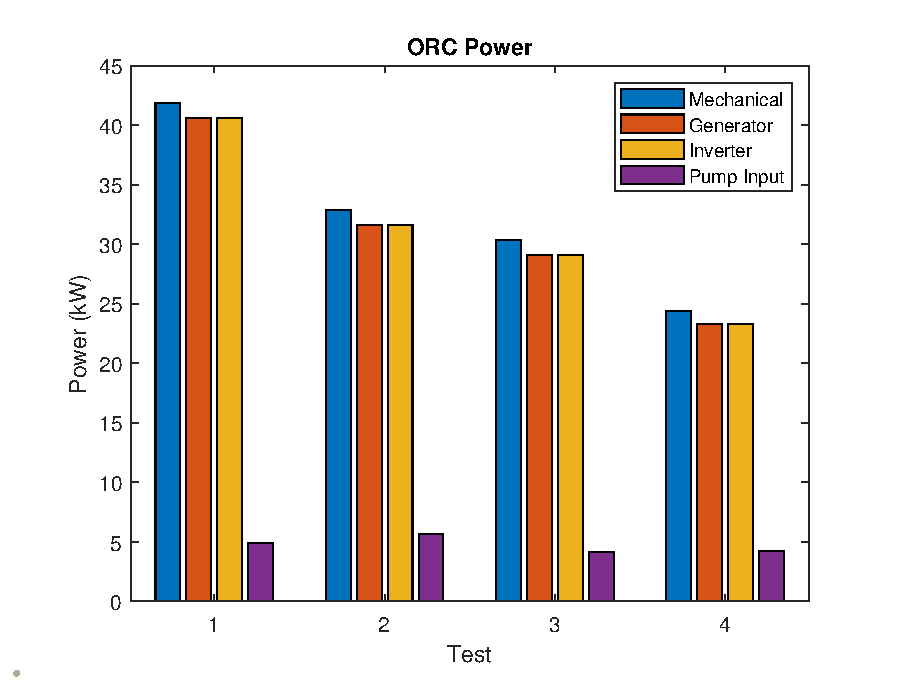
\includegraphics[width=\textwidth]{figures/VerificationPower01}
	%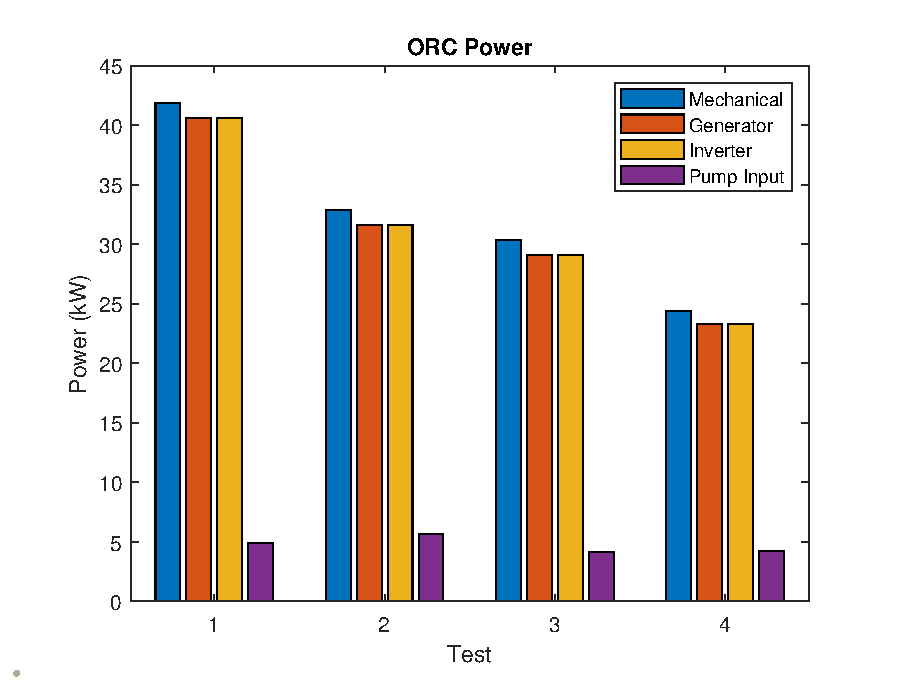
\includegraphics[width=0.5\textwidth]{figures/VerificationPower01}
	
	\caption{Comparison of mechanical power, generator power, inverter output power, and pump power consumption for the validation of the ORC prime power system model. All tests assume a sink temperature of \SI{283}{\kelvin} (\SI{10}{\degreeCelsius}). Tests 1 and 2 use a heat source temperature of \SI{364}{\kelvin} (\SI{91}{\degreeCelsius}), while tests 3 and 4 use \SI{353}{\kelvin} (\SI{79}{\degreeCelsius}). Tests 1 and 3 use a source flow rate of \SI{19}{\liter\per\second} and a sink flow rate of \SI{13}{\liter\per\second}, where as tests 3 and 4 use a source and sink flow rate of \SI{8}{\liter\per\second}.
	%The power setpoints of the four tests are \SIlist{27.5;40.0;30.8;42.0}{\kilo\watt}. Tests 1 and 3 use the maximum power setpoint while also ensuring the working fluid fully evaporates in the evaporator. Tests 2 and 4, use the maximum power setpoint while maintaining a stable simulation. 
	}
	%Psetpoint[2.75e4;4.0e4;3.08e4;4.2e4;]
	\label{fig:verificationPower01}
\end{figure}
\begin{figure}[h]
	\centering
	
	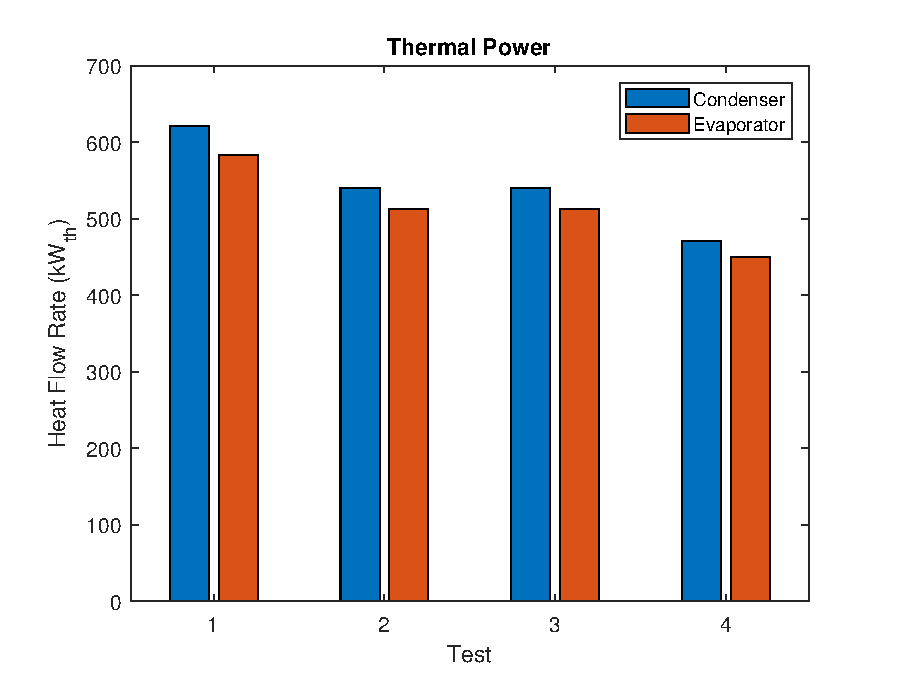
\includegraphics[width=\textwidth]{figures/VerificationHeat01}
	%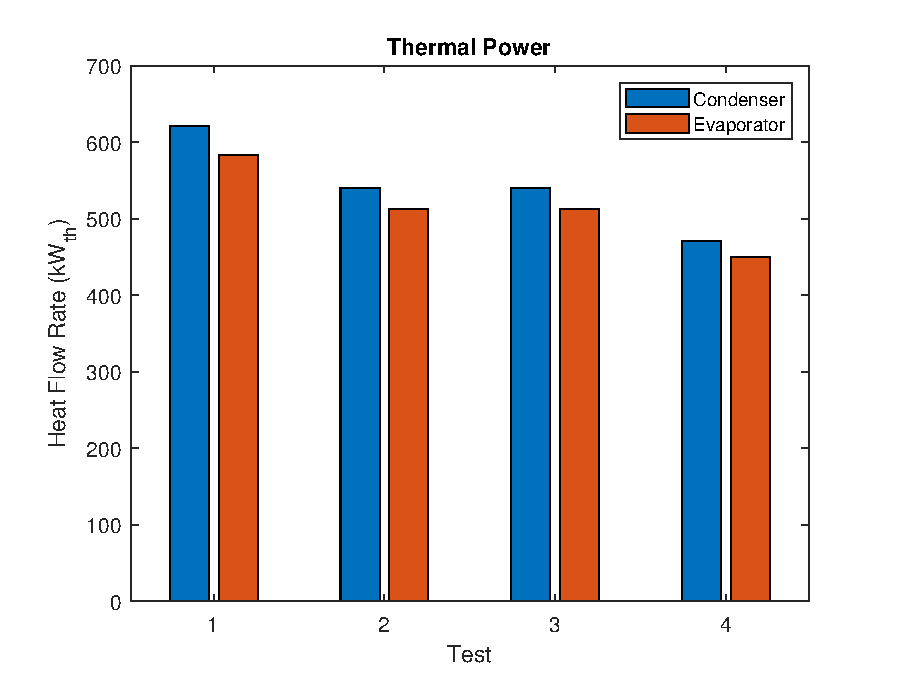
\includegraphics[width=0.5\textwidth]{figures/VerificationHeat01}
	
	\caption{Comparison of evaporator and condenser heat flow rates for the validation of the ORC prime power system model. All tests assume a sink temperature of \SI{283}{\kelvin} (\SI{10}{\degreeCelsius}). Tests 1 \& 2 use a heat source temperature of \SI{364}{\kelvin} (\SI{91}{\degreeCelsius}), while tests 3 \& 4 use \SI{353}{\kelvin} (\SI{79}{\degreeCelsius}). Tests 1 \& 3 use a source flow rate of \SI{19}{\liter\per\second} and a sink flow rate of \SI{13}{\liter\per\second}, where as test 3 \& 4 use a source and sink flow rate of \SI{8}{\liter\per\second}.
	%The power setpoints of the four tests are \SIlist{27.5;40.0;30.8;42.0}{\kilo\watt}. Tests 1 \& 3 use the maximum power setpoint while also ensuring the working fluid fully evaporates in the evaporator. Tests 2 \& 4, use the maximum power setpoint while maintaining a stable simulation. 
	}
	%Psetpoint[2.75e4;4.0e4;3.08e4;4.2e4;]
	\label{fig:verificationHeat01}
\end{figure}
\begin{figure}[p]
	\centering
	
	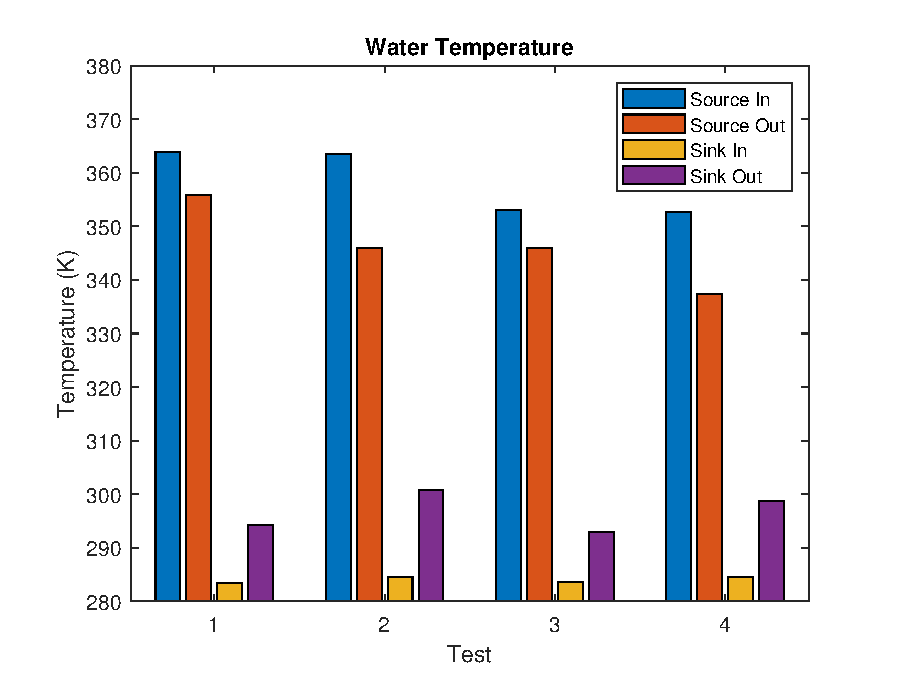
\includegraphics[width=\textwidth]{figures/VerificationWaterTemp01}
	%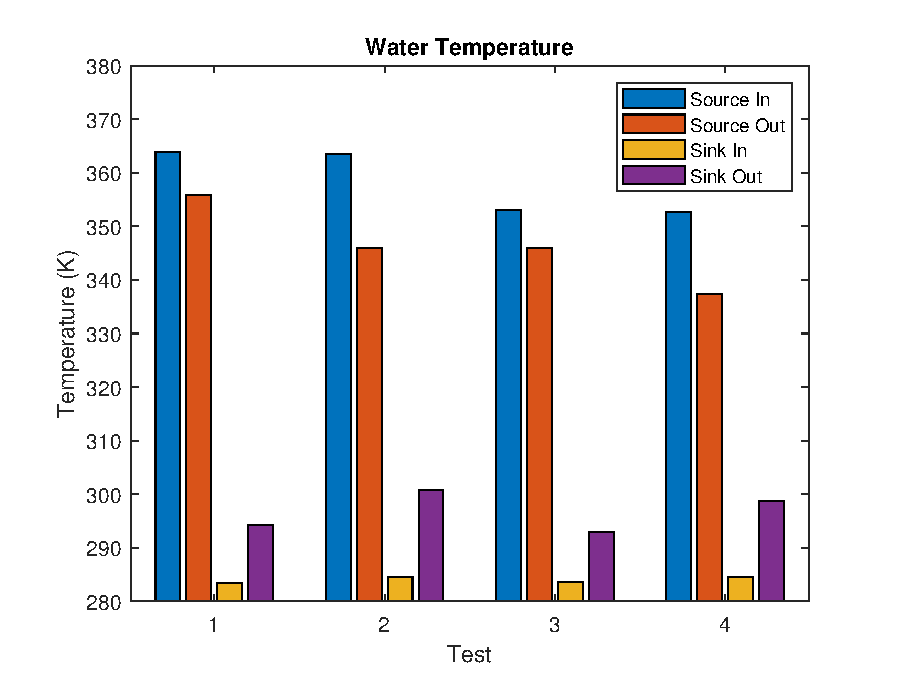
\includegraphics[width=0.5\textwidth]{figures/VerificationWaterTemp01}
	
	\caption{Comparison of source and sink inlet and outlet temperatures for the validation of the ORC prime power system model. All tests assume a sink temperature of \SI{283}{\kelvin} (\SI{10}{\degreeCelsius}). Tests 1 and 2 use a heat source temperature of \SI{364}{\kelvin} (\SI{91}{\degreeCelsius}), while tests 3 and 4 use \SI{353}{\kelvin} (\SI{79}{\degreeCelsius}). Tests 1 and 3 use a source flow rate of \SI{19}{\liter\per\second} and a sink flow rate of \SI{13}{\liter\per\second}, where as tests 3 and 4 use a source and sink flow rate of \SI{8}{\liter\per\second}.
	%The power setpoints of the four tests are \SIlist{27.5;40.0;30.8;42.0}{\kilo\watt}. Tests 1 and 3 use the maximum power setpoint while also ensuring the working fluid fully evaporates in the evaporator. Tests 2 and 4, use the maximum power setpoint while maintaining a stable simulation. 
	}
	%Psetpoint[2.75e4;4.0e4;3.08e4;4.2e4;]
	\label{fig:verificationWaterTemp01}
\end{figure}

As desired, the gross electrical power output of the model matches the measured value for each set of inputs. However, the power consumed to run the pump is a factor of 2-3 times greater in the model than what was measured. A pump sizing guide \cite{CheGuide2017} was used to calculate hypothetical hydraulic power needed to move a liquid at the density of R245-fa across each of the pressure differences listed at the corresponding flow rates. When these hydraulic power values have the assumed pump and drive efficiencies applied as well, they match the pump power values of the model. This indicates the working fluid flow rates of the model are much greater than the operating values measured during the Green Machine ORC system test.

The calculated heat transferred in both the evaporator and the condenser are greater than what was measured in each case. Although the values do tend to follow a similar pattern with higher source temperatures and water flow rates resulting in greater rates of heat transferred. Additionally, the source and sink fluids undergo a greater temperature change in the model as a result of the higher heat flow rates.


%The likely reason for the difference in heat flows is model assumes all the heat flows from one fluid to another and does not affect the ambient temperature. This is also a possible explanation for higher pump power consumptions seen in the model. With both more heat being added and removed from the working fluid, but the same amount of mechanical power being extracted from it, the fluid is likely being 

Pressure was plotted against enthalpy at various points of the cycle in \autoref{fig:verifcation_ph01} for each of the four tests. The two curves indicate the pressure-enthalpy combinations of R245-fa where the working fluid begins to condense and vaporize. The top-left group of points represents the working fluid at the outlet of the pump. The top-right group represents the working fluid at the inlet of the expander. The bottom-right group represents the working fluid at the outlet of the expander. Finally, The bottom-left group represents the working fluid at the inlet of the pump.
\begin{figure}[h]
	\centering

	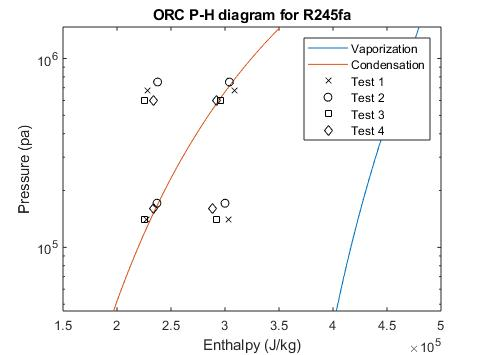
\includegraphics[width=\textwidth]{figures/VerificationPH01}
	%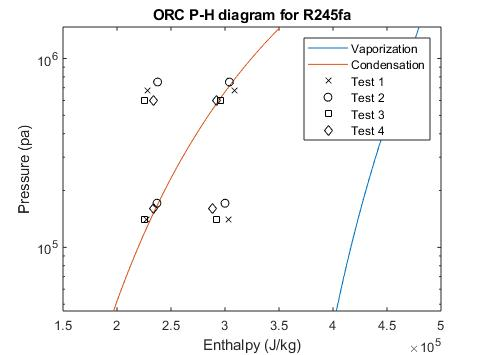
\includegraphics{figures/VerificationPH01}

	\caption{Pressure-Enthalpy plot of R245-fa for ORC verification. 
	For tests 1 \& 2 $T_{source}$ is about \SI{364}{\kelvin} (\SI{195}{\degreeFahrenheit})
	while for 3 \& 4 $T_{source}$ is \SI{353}{\kelvin} (\SI{175}{\degreeFahrenheit}). 
	In all cases $T_{sink}$ is about \SI{283}{\kelvin} (\SI{50}{\degreeFahrenheit}). 
	The hot water flow rate for tests 1 \& 3 are \SI{18.9}{\liter\per\second} (\SI{300}{\gpm})
	and	\SI{7.6}{\liter\per\second} (\SI{120}{\gpm}) for test 2 \& 4. 
	The cold water flow rate for tests 1 \& 3 are \SI{12.6}{\liter\per\second} (\SI{200}{\gpm})
	and \SI{7.6}{\liter\per\second} (\SI{120}{\gpm}) for test 2 \& 4.}
	\label{fig:verifcation_ph01}
\end{figure}

For each of these tests, the working fluid just barely begins to boil in the evaporator, if at all. It is expected that the working fluid will either completely vaporize, or at least be further to the right in the liquid-vapor region. Along with the higher than expected pump power, this also indicates that there is more working fluid being pumped throughout the cycle in the model than what was measured.

To re-create conditions where the system outputs comparable between the modeled and measured values while pumping less fluid, the evaporator area is increased by a factor of four so it is comparable to the area of the condenser. Additionally, the pressure set points are adjusted to values seen in \autoref{tab:verification_ORC_vars02} to account for the new temperatures of the working fluid.
\begin{table}%[h]
	\centering
	\caption{Input variables for the verification of the Organic Rankine Cycle Model.}
	%\rowcolors{5}{}{gray!10}
	\label{tab:verification_ORC_vars02}
	\begin{tabular}{rllll}
		\toprule
		                                              &  Case &       &       &       \\ \cline{2-5}
		                                              &     1 &     2 &     3 &     4 \\ \midrule

		$p_{hi}(\si{\kilo\pascal})  $                 &  0.68 &  0.75 &  0.60 &  0.60 \\
		$p_{low}(\si{\kilo\pascal}) $                 &  0.14 &  0.17 &  0.14 &  0.16 \\
%		$P_{setpoint}(\si{\kilo\watt})$               &  34.7 &  27.1 &  24.6 &  19.0 \\ 
		\bottomrule
	\end{tabular}
\end{table}



The results of the second set of validation tests are plotted in \autoref{fig:verificationPower02} for the power values, \autoref{fig:verificationHeat02} for the heat flow rate values, and \autoref{fig:verificationWaterTemp02} for the water temperature values. \autoref{tab:verification_results02} compares the simulation results with the measured results. As expected, the gross output power remained roughly equal to the measured values. The consumed pump power decreased significantly in the new set of tests. Those values are now about half the measured ones, indicating the fluid is moving at a slower rate. The thermal power measurements are now greater than the simulated values by about \SIrange{30}{80}{\kilo\watt\textsubscript{th}} and the source and sink outlet temperatures are correspondingly higher and lower, respectively. \autoref{fig:verifcation_ph02} shows the lower mass flow rate of the working fluid allows it to fully vaporize due to the larger transfer area of the evaporator. 
\begin{table}%[h]
	\centering
	\caption{Comparison of output variables for the verification of the ORC Model with modified evaporator area.}
	%\rowcolors{5}{}{gray!10}
	\label{tab:verification_results02}
	\begin{tabular}{rllllllll}
		\toprule
		                                           & Case  &       &       &       &       &       &       &       \\ \cline{2-9}
		                                           & 1     &       & 2     &       & 3     &       & 4     &       \\
		                                           & Meas. & Model & Meas. & Model & Meas. & Model & Meas. & Model \\ \midrule
		              $P_{gross}(\si{\kilo\watt})$ & 40.7  & 40.7  & 31.8  & 31.9  & 29.2  & 29.2  & 22.7  & 22.5  \\
		               $P_{pump}(\si{\kilo\watt})$ & 2.6   & 1.1   & 1.9   & 0.92  & 1.5   & 0.72  & 1.3   & 0.55  \\
		            %$P_{source}(\si{\kilo\watt})$ & 9.6   & -     & 1.0   & -     & 10.0  & -     & 1.0   & -     \\
		              %$P_{sink}(\si{\kilo\watt})$ & 3.5   & -     & 1.0   & -     & 3.5   & -     & 1.0   & -     \\
		              $P_{evap.}(\si{\kilo\watt})$ & 519   & 441   & 413   & 340   & 393   & 364   & 328   & 277   \\
		              $P_{cond.}(\si{\kilo\watt})$ & 464   & 400   & 385   & 307   & 356   & 335   & 303   & 254   \\
		            $T_{source,out}(\si{\kelvin})$ & 357.2 & 358.2 & 350.1 & 352.5 & 347.9 & 348.2 & 342.0 & 343.7 \\
		              $T_{sink,out}(\si{\kelvin})$ & 292.1 & 290.9 & 296.9 & 294.4 & 290.1 & 289.7 & 294.2 & 292.6 \\ \bottomrule
		          %$P_{setpoint}(\si{\kilo\watt})$ &       &       &       &       &       &       &       &       \\
		%$\dot{m}_{wf}(\si{\kilogram\per\second})$ & -     &       & -     &       & -     &       & -     &
	\end{tabular}
\end{table}


\begin{figure}[h]
	\centering
	
	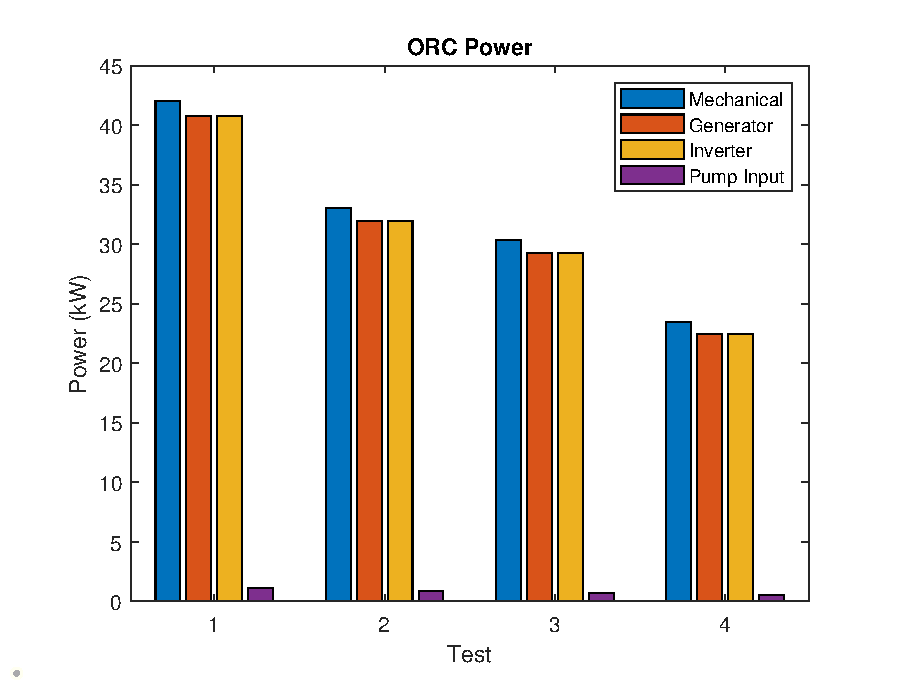
\includegraphics[width=\textwidth]{figures/VerificationPower02}
	%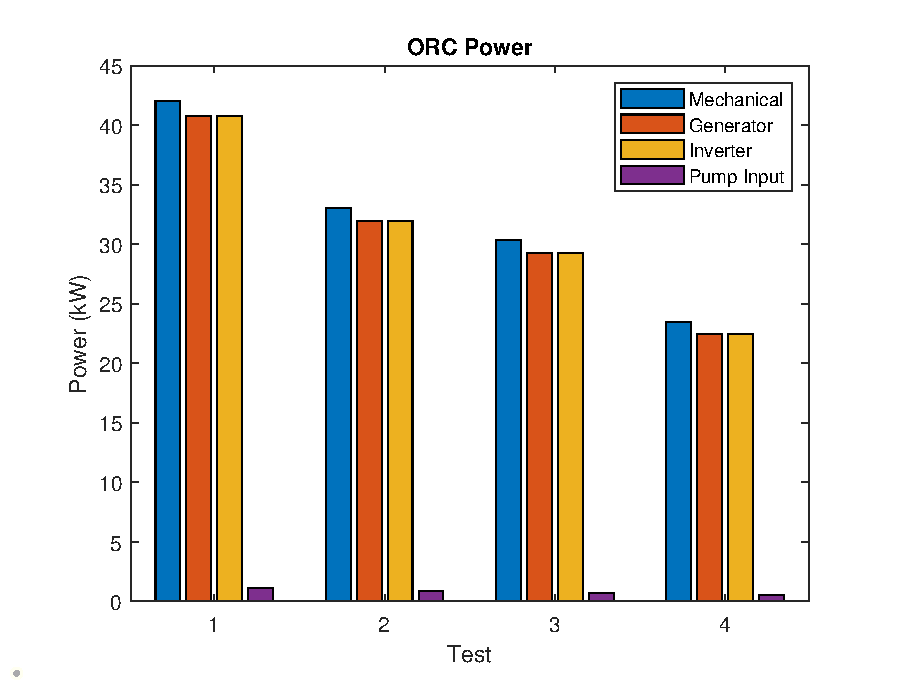
\includegraphics[width=0.5\textwidth]{figures/VerificationPower02}
	
	\caption{Comparison of mechanical power, generator power, inverter output power, and pump power consumption for the validation of the ORC prime power system model with an increased evaporator area. All tests assume a sink temperature of \SI{283}{\kelvin} (\SI{10}{\degreeCelsius}). Tests 1 \& 2 use a heat source temperature of \SI{364}{\kelvin} (\SI{91}{\degreeCelsius}), while tests 3 \& 4 use \SI{353}{\kelvin} (\SI{79}{\degreeCelsius}). Tests 1 \& 3 use a source flow rate of \SI{19}{\liter\per\second} and a sink flow rate of \SI{13}{\liter\per\second}, where as test 3 \& 4 use a source and sink flow rate of \SI{8}{\liter\per\second}.
	%The power setpoints of the four tests are \SIlist{27.5;40.0;30.8;42.0}{\kilo\watt}. Tests 1 \& 3 use the maximum power setpoint while also ensuring the working fluid fully evaporates in the evaporator. Tests 2 \& 4, use the maximum power setpoint while maintaining a stable simulation. 
	}
	%Psetpoint[2.75e4;4.0e4;3.08e4;4.2e4;]
	\label{fig:verificationPower02}
\end{figure}
\begin{figure}[p]
	\centering
	
	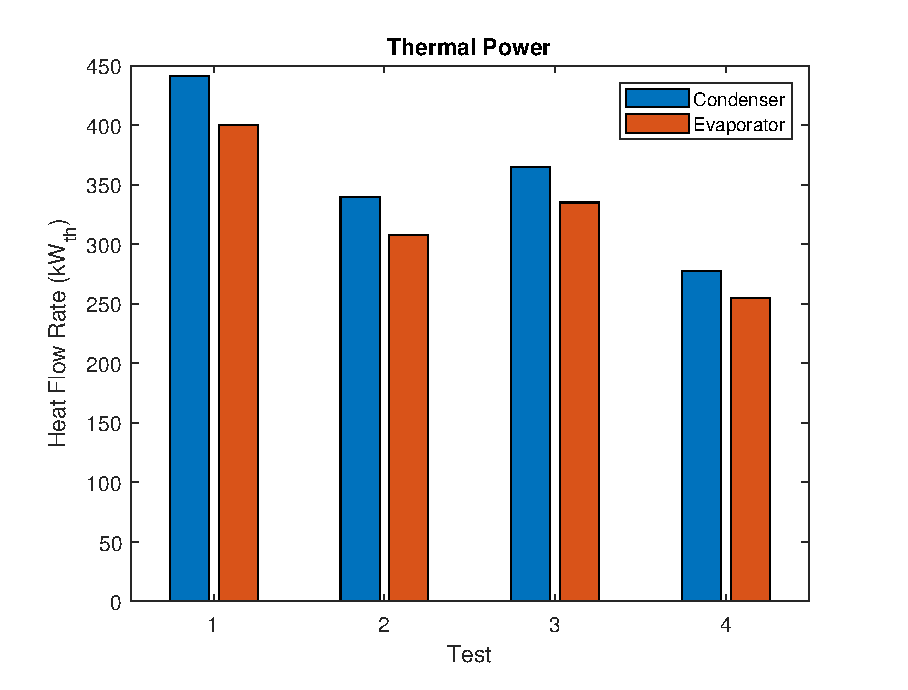
\includegraphics[width=\textwidth]{figures/VerificationHeat02}
	%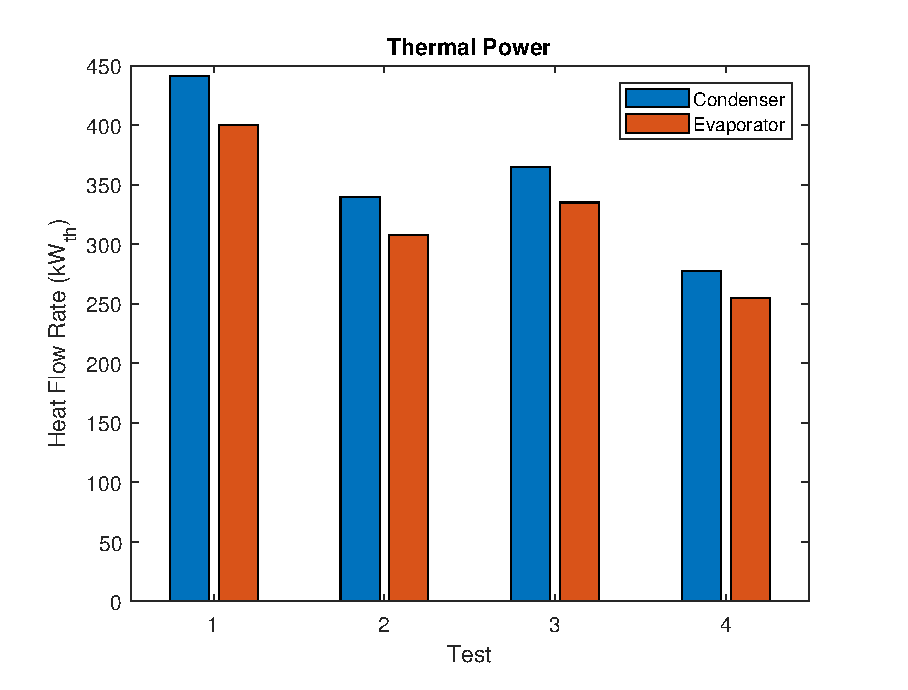
\includegraphics[width=0.5\textwidth]{figures/VerificationHeat02}
	
	\caption{Comparison among evaporator and condenser heat flow rates for the validation of the ORC prime power system model with an increased evaporator area. All tests assume a sink temperature of \SI{283}{\kelvin} (\SI{10}{\degreeCelsius}). Tests 1 and 2 use a heat source temperature of \SI{364}{\kelvin} (\SI{91}{\degreeCelsius}), while tests 3 and 4 use \SI{353}{\kelvin} (\SI{79}{\degreeCelsius}). Tests 1 and 3 use a source flow rate of \SI{19}{\liter\per\second} and a sink flow rate of \SI{13}{\liter\per\second}, where as tests 3 and 4 use a source and sink flow rate of \SI{8}{\liter\per\second}.
	%The power setpoints of the four tests are \SIlist{27.5;40.0;30.8;42.0}{\kilo\watt}. Tests 1 and 3 use the maximum power setpoint while also ensuring the working fluid fully evaporates in the evaporator. Tests 2 and 4, use the maximum power setpoint while maintaining a stable simulation. 
	}
	%Psetpoint[2.75e4;4.0e4;3.08e4;4.2e4;]
	\label{fig:verificationHeat02}
\end{figure}
\begin{figure}[h]
	\centering
	
	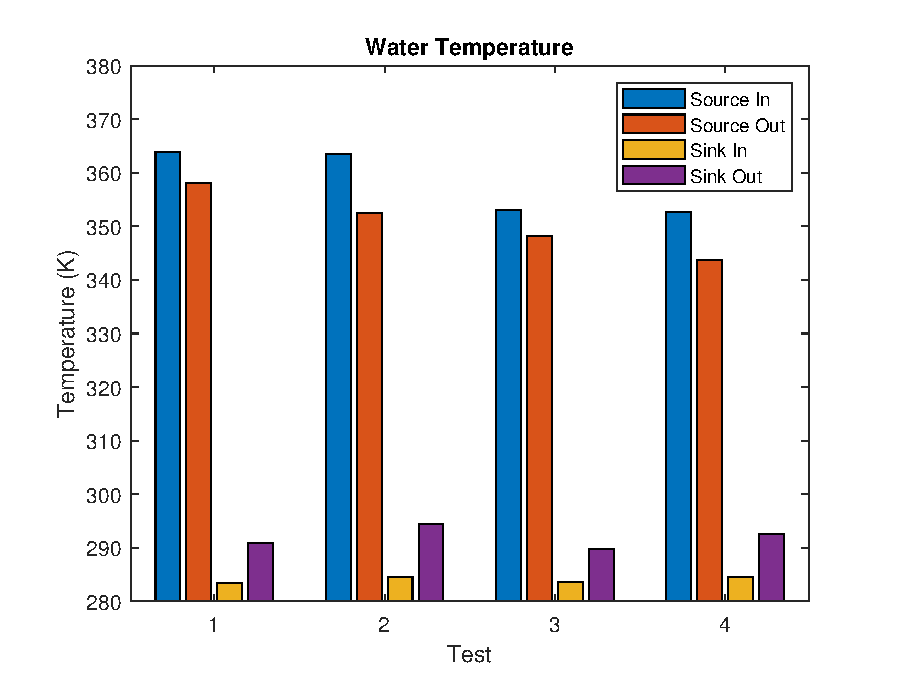
\includegraphics[width=\textwidth]{figures/VerificationWaterTemp02}
	%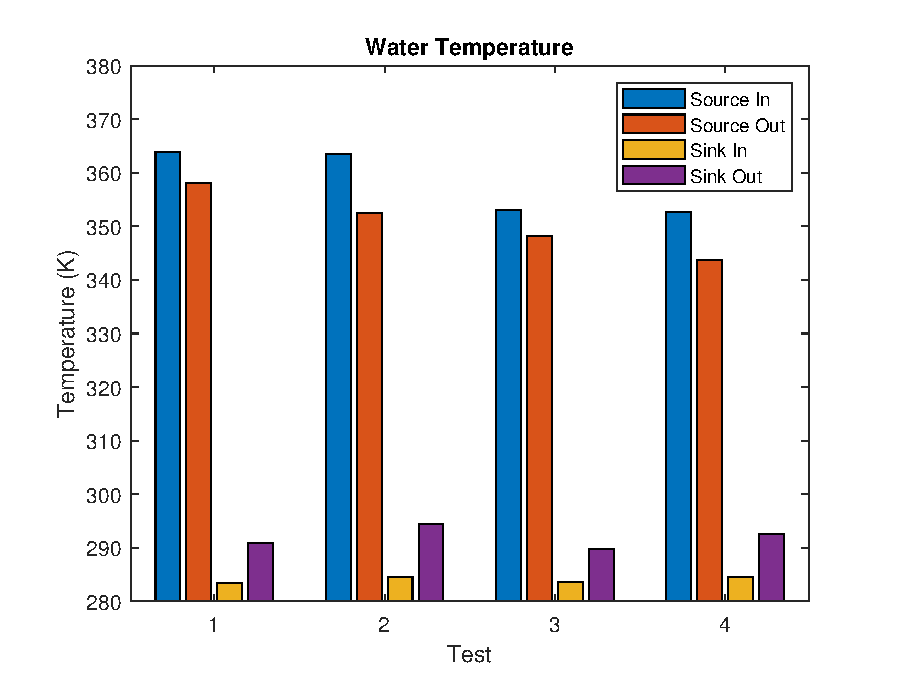
\includegraphics[width=0.5\textwidth]{figures/VerificationWaterTemp02}
	
	\caption{Comparison of source and sink inlet and outlet temperatures for the validation of the ORC prime power system model with an increased evaporator area. All tests assume a sink temperature of \SI{283}{\kelvin} (\SI{10}{\degreeCelsius}). Tests 1 \& 2 use a heat source temperature of \SI{364}{\kelvin} (\SI{91}{\degreeCelsius}), while tests 3 \& 4 use \SI{353}{\kelvin} (\SI{79}{\degreeCelsius}). Tests 1 \& 3 use a source flow rate of \SI{19}{\liter\per\second} and a sink flow rate of \SI{13}{\liter\per\second}, where as test 3 \& 4 use a source and sink flow rate of \SI{8}{\liter\per\second}.
	%The power setpoints of the four tests are \SIlist{27.5;40.0;30.8;42.0}{\kilo\watt}. Tests 1 \& 3 use the maximum power setpoint while also ensuring the working fluid fully evaporates in the evaporator. Tests 2 \& 4, use the maximum power setpoint while maintaining a stable simulation. 
	}
	%Psetpoint[2.75e4;4.0e4;3.08e4;4.2e4;]
	\label{fig:verificationWaterTemp02}
\end{figure}
\begin{figure}%[h]
	\centering
	\caption{Pressure-Enthalpy plot of R245-fa for ORC verification with an over sized evaporator area. Input tempetures and flow rates remain the same. 
	For tests 1 \& 2 $T_{source}$ is about \SI{364}{\kelvin} (\SI{195}{\degreeFahrenheit})
	while for 3 \& 4 $T_{source}$ is \SI{353}{\kelvin} (\SI{175}{\degreeFahrenheit}). 
	In all cases $T_{sink}$ is about \SI{283}{\kelvin} (\SI{50}{\degreeFahrenheit}). 
	The hot water flow rate for tests 1 \& 3 are \SI{18.9}{\liter\per\second} (\SI{300}{\gpm})
	and	\SI{7.6}{\liter\per\second} (\SI{120}{\gpm}) for test 2 \& 4. 
	The cold water flow rate for tests 1 \& 3 are \SI{12.6}{\liter\per\second} (\SI{200}{\gpm})
	and \SI{7.6}{\liter\per\second} (\SI{120}{\gpm}) for test 2 \& 4.}
	\label{fig:verifcation_ph02}
	
	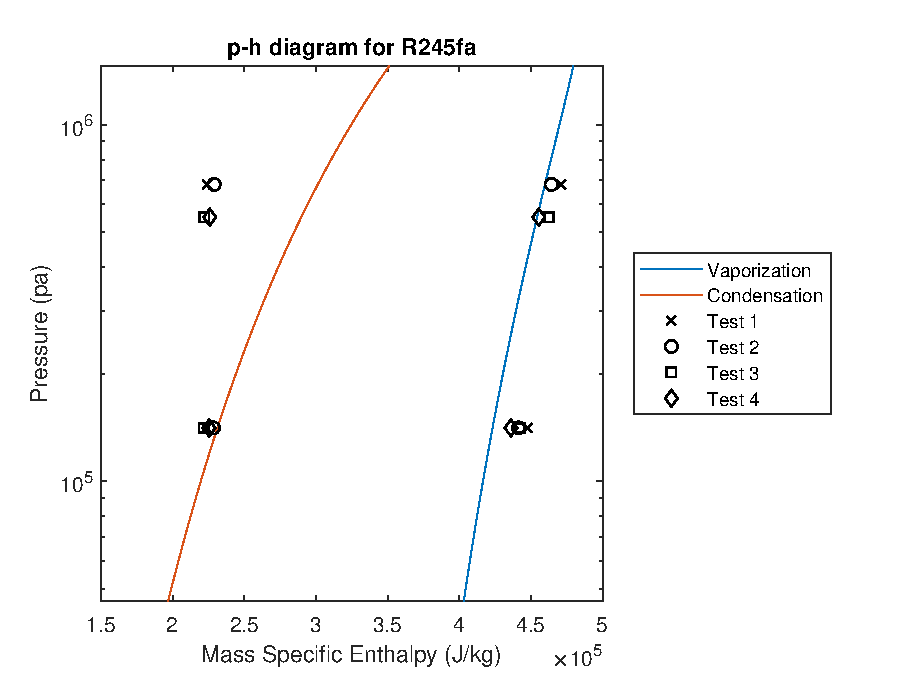
\includegraphics[width=\textwidth]{figures/VerificationPH02}
	%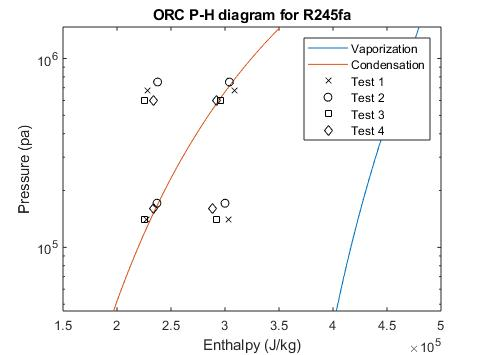
\includegraphics{figures/VerificationPH01}
\end{figure}

Under four different combinations of source and sink flow rates and temperatures, the gross output power of the model matched the measured values. However, given the assumed heat transfer area of the evaporator and condenser, the power consumed by the pump was calculated to be much greater than what was measured. Increasing the area of the evaporator such that it roughly matched the condenser greatly reduced the calculated power needed by the pump. However, this is not typical for ORCs. Generally condensers are sized larger than evaporators so the system can also feasibly use air to cool the working fluid. 
\clearpage

\section{Case Study Scenarios}
With the model validated the Greenfield and Brownfield scenarios can be simulated and analyzed. For the former, no electrical grid is currently present, while for the later there is existing electrical infrastructure. However, in the brownfield case the grid is not perfectly reliable. In the event of a grid outage, the microgrid should be capable of disconnecting and acting on its own. In both scenarios, the same generator impedances are used as in the validation simulations. 

\subsection{Greenfield Scenario --- Alaska}
This system is located approximately two hours north of Nome, Alaska on the western coast of the state. The hot water resource is drawn from the Pilgrim Hot Springs. The hot water is assumed to be drawn at a temperature of \SI{364.5}{\kelvin} (\SI{91.3}{\degreeCelsius}) and a flow rate of \SI{15.2}{\liter\per\second}. The hot water resource is fairly stable throughout the year. The low temperature water ranges from \SIrange{276.6}{281.6}{\kelvin} (\SIrange{3.5}{8.5}{\degreeCelsius}) at a flow rate of \SI{15.6}{\liter\per\second} to provide a heat sink \cite{Haselwimmer2013, AlaskaCenterforEnergyandPower2014}. Though the low temperature sink resource does vary in temperature with the seasons, the nearby geothermal activity keeps it liquid all year round.
%It is assumed the water is drawn in at atmospheric pressure.

The assumed working fluid is R245-fa, a typical refrigerant used by ORC manufacturers such as Electratherm, Clean Energy Technologies Inc., etc. The operating high and low pressure set points of the working fluid are \SIrange{570}{600}{\kilo\pascal} and \SIrange{130}{140}{\kilo\pascal}, respectively. The evaporator has a heat transfer area of \SI{37.8}{\meter\squared}, and an effective heat transfer coefficient of \SI{1500}{\watt\per\kelvin\per\meter\squared}. The condenser has an area of \SI{102.5}{\meter\squared}, but an effective heat transfer coefficient of \SI{1400}{\watt\per\kelvin\per\meter\squared}.

Four tests were conducted under different input conditions. Tests one and two use the warmer summer heat sink temperature, while tests three and four use the colder winter heat sink temperatures. Furthermore, tests one and three use the maximum power setpoint while also ensuring the working fluid fully evaporates in the evaporator, whereas in tests two and four, the power setpoint increased to the maximum value while maintaining a stable simulation. \autoref{fig:gfPower} compares the mechanical power, $P_{mech}$, the generator power, $P_{gen}$, inverter output power, $P_{out}$, and the electrical power consumed by the pump, $P_{pump}$ of the different tests. The working fluid mass flow rates, $\dot{m}$, are seen in \autoref{fig:gfFlow}. Finally, the heat flow rates of the evaporator and condenser, $\dot{Q}_{evap}$ and $\dot{Q}_{cond}$, are seen in \autoref{fig:gfHeat}.
\begin{figure}[p]
	\centering

	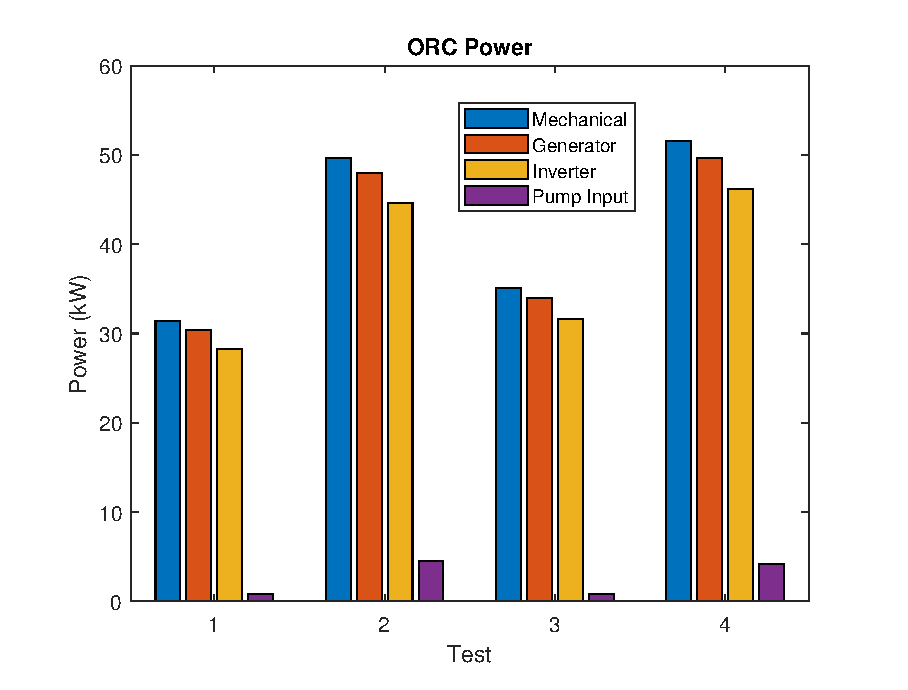
\includegraphics[width=\textwidth]{figures/gfPower}

	\caption{Comparison of mechanical power, generator power, inverter output power, and pump power consumption for the greenfield case of the ORC prime power system model. All tests assume a source temperature of \SI{364.5}{\kelvin} (\SI{91}{\degreeCelsius}), and source and sink flow rates of \SI{940}{\liter\per\minute}. Tests 1 and 2 use a heat sink temperature of \SI{281.6}{\kelvin} (\SI{8.5}{\degreeCelsius}), while tests 3 and 4 use \SI{276.6}{\kelvin} (\SI{3.5}{\degreeCelsius}). The power setpoints of the four tests are \SIlist{27.5;40.0;30.8;42.0}{\kilo\watt}. Tests 1 and 3 use the maximum power setpoint while also ensuring the working fluid fully evaporates in the evaporator. Tests 2 and 4 use the maximum power setpoint while maintaining a stable simulation. }
	%Psetpoint[2.75e4;4.0e4;3.08e4;4.2e4;]
	\label{fig:gfPower}
\end{figure}
\begin{figure}[p]
	\centering

	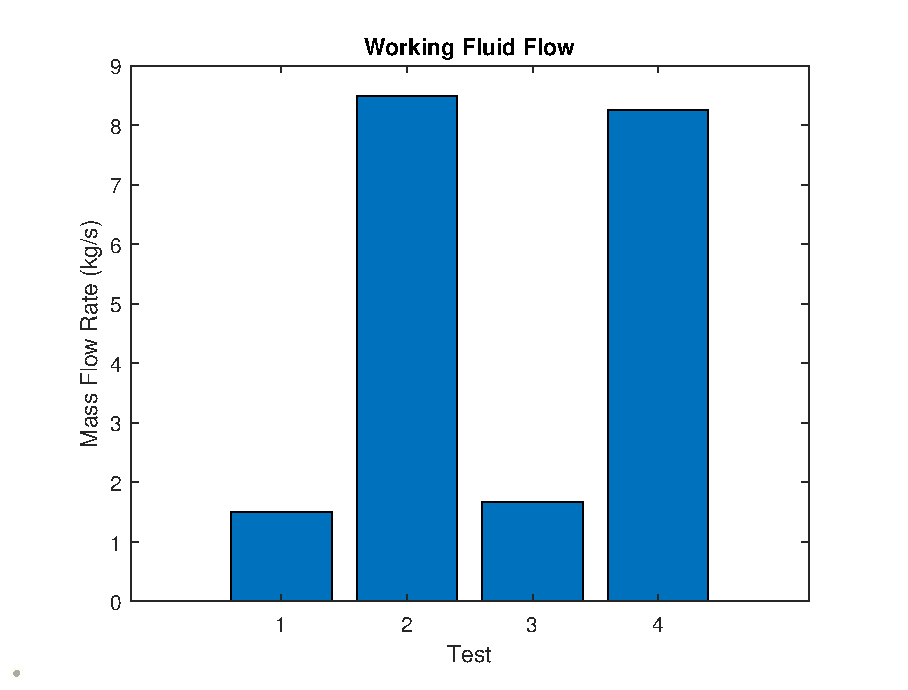
\includegraphics[width=\textwidth]{figures/gfFlow}

	\caption{Comparison of working fluid mass flow rates for the greenfield case of the ORC prime power system model. All test assume a source temperatures of \SI{364.5}{\kelvin} (\SI{91}{\degreeCelsius}), and source and sink flow rates of \SI{940}{\liter\per\minute}. Tests 1 and 2 use a heat sink temperature of \SI{281.6}{\kelvin} (\SI{8.5}{\degreeCelsius}), while tests 3 and 4 use \SI{276.6}{\kelvin} (\SI{3.5}{\degreeCelsius}). The power setpoints of the four tests are \SIlist{27.5;40.0;30.8;42.0}{\kilo\watt}. Tests 1 and 3 use the maximum power setpoint while also ensuring the working fluid fully evaporates in the evaporator. Tests 2 and 4 use the maximum power setpoint while maintaining a stable simulation. }
	%Psetpoint[2.75e4;4.0e4;3.08e4;4.2e4;]
	\label{fig:gfFlow}
\end{figure}
\begin{figure}[p]
	\centering

	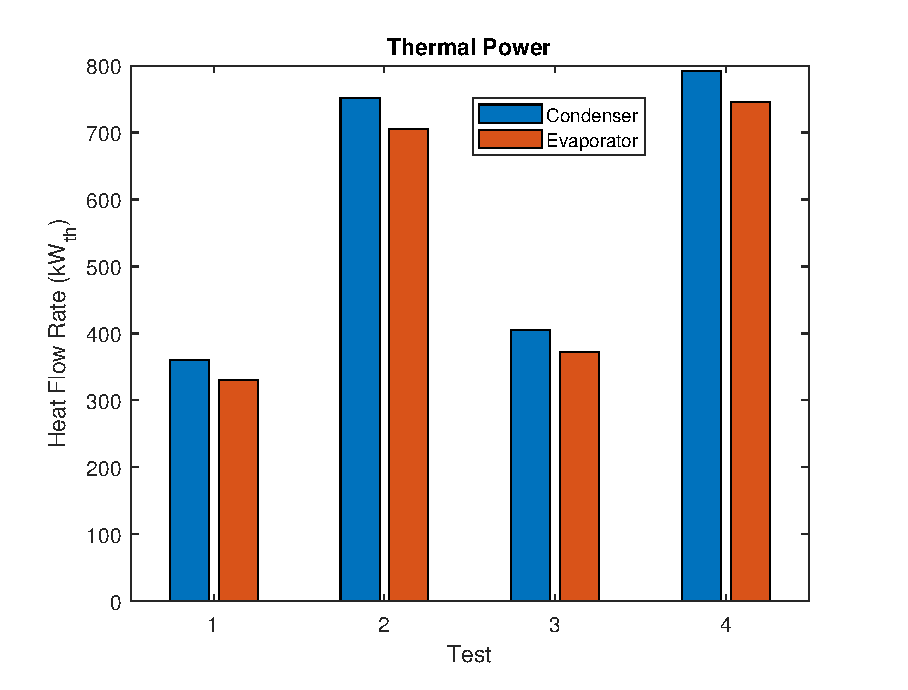
\includegraphics[width=\textwidth]{figures/gfHeat}

	\caption{Comparison among heat flow rates through the evaporator and condenser for the greenfield ORC prime power system model. All test assume a source temperatures of \SI{364.5}{\kelvin} (\SI{91}{\degreeCelsius}), and source and sink flow rates of \SI{940}{\liter\per\minute}. Tests 1 and 2 use a heat sink temperature of \SI{281.6}{\kelvin} (\SI{8.5}{\degreeCelsius}), while tests 3 and 4 use \SI{276.6}{\kelvin} (\SI{3.5}{\degreeCelsius}). The power setpoints of the four tests are \SIlist{27.5;40.0;30.8;42.0}{\kilo\watt}. Tests 1 and 3 use the maximum power setpoint while also ensuring the working fluid fully evaporates in the evaporator. Tests 2 and 4 use the maximum power setpoint while maintaining a stable simulation. }
	%Psetpoint[2.75e4;4.0e4;3.08e4;4.2e4;]
	\label{fig:gfHeat}
\end{figure}

Depending on the operator's tolerance of the state of the working fluid, the available gross output of the ORC prime power system can vary significantly. The gross output power of the inverter, $P_{out}$, the system can achieve while ensuring the working fluid fully vaporizes is \SIrange{28.3}{31.6}{\kilo\watt} throughout the year. In these cases the pump only needs to move about \SI{1.6}{\kilogram\per\second} consuming \SI{0.80}{\kilo\watt}. This yields a net output of \SIrange{27.5}{30.8}{\kilo\watt} before accounting for the power required for hot and cold water pumps. Heat is absorbed from hot water at a rate, $\dot{Q}_{evap}$, of \SIrange{361}{406}{\kilo\watt\textsubscript{th}} indicating a net efficiency of $\eta = 7.6\%$, where $\eta = \frac{P_{out}-P_{pump}}{\dot{Q}_{evap}}$.

More heat can be moved by increasing the working fluid flow rate yielding a greater gross output. For flow rates of around \SI{8.4}{\kilogram\per\second}, the gross output of the system is \SIrange{44.6}{46.2}{\kilo\watt}, with the greater end of the range occurring during the winter. Under these conditions the pump consumes about \SI{4.5}{\kilo\watt} cycling the working fluid, netting an output of \SIrange{40.1}{41.7}{\kilo\watt}. More power is being generated because heat is being transferred at a greater rate from the source, \SIrange{751}{792}{\kilo\watt\textsubscript{th}}, but the efficiency is lower at about 5.3\%.

The drop in efficiency from 7.6\% to 5.3\% as the working fluid flow rate increases can be understood by the plots in \autoref{fig:gf_themoplots}. The curves represent the dividing lines between pure liquid, pure gaseous, and the in-between state. The points represent the state of the working fluid between each block for the four different tests: low working fluid flow rate during summer, high flow rate during summer, low flow rate in winter, and high flow rate in winter. 
\begin{figure}%[h]
	\centering
	\caption{Thermodynamic plots of the simulated greenfield ORC plotting pressure against temperature, pressure against enthalpy, and temperature against entropy. All points assume a source temperatures of \SI{91}{\degreeCelsius}, and source and sink flow rates of \SI{940}{\liter\per\minute}. Winter sink temperatures are assumed to be \SI{3.5}{\degreeCelsius} while summer source temperatures are \SI{8.5}{\degreeCelsius}. High flow rate points have a working fluid mass flow rate of approximately \SI{8.4}{\kilogram\per\second}}
	\label{fig:gf_themoplots}
	
	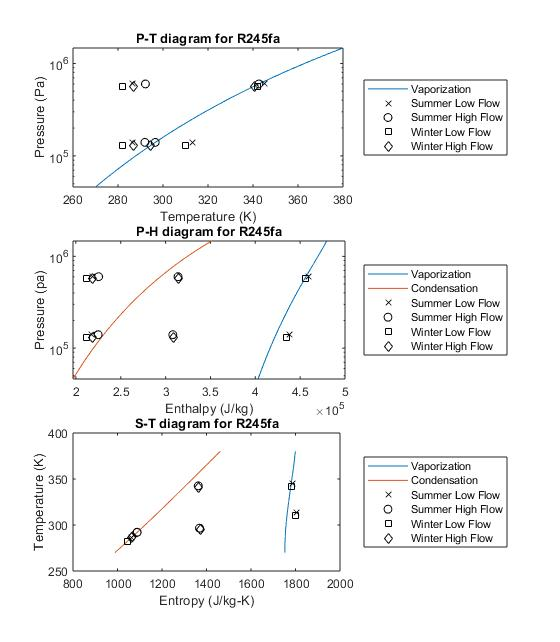
\includegraphics[width=\textwidth]{figures/GreenfieldThermoPlots}
	%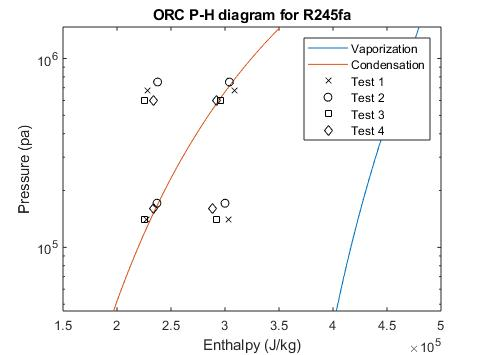
\includegraphics{figures/VerificationPH01}
\end{figure}

The first plot shows pressure (\si{\pascal}) versus temperature (\si{\kelvin}). A benefit of this plot is that it is easy to identify increases and decreases in both temperature and pressure as the working fluid moves through the cycle. However, this comes a cost of resolution in the liquid-vapor region. In this plot the vaporization and condensation curve overlap without representing the latent heat needed to change from one phase to the other. In this particular plot there are points in this area that are not discernible despite being at different energy levels. 

The second plot helps resolve this problem by plotting enthalpy (\si[per-mode=symbol-or-fraction]{\joule\per\kilogram}) on the x-axis instead of temperature. It can be seen that the low flow rate tests allow the fluid to fully become a gas and cross the vaporization curve. Since each \si{\kilogram} of fluid contains more energy, the turbine is able to operate more efficiently, even though more total energy is being extracted at higher flow rates.

The third and final plot of \autoref{fig:gf_themoplots} plots temperature (\si{\kelvin}) against mass specifc entropy (\si[per-mode=symbol-or-fraction]{\joule\per\kilogram\per\kelvin}). This shows the non-ideal isentropic transition of the pump and turbine. This is difficult to see for the pump because the points before and after the pump lie nearly on top of one another. Both the temperature and entorpy changed very little in the process. In the turbine, however, it is clearer. Ideally the points would drop straight down on this plot, but instead there is a slight increase in entropy due to the isentropic inefficiency, as expected from the 2\textsuperscript{nd} law of thermodynamics. 

The \SI{30.8}{\kilo\watt} output could be used to operate a greenhouse nearby during the winter. Assuming about \SI{1}{\kilo\watt} of power to supply the circulation fans and watering system, as well as LED lighting of 
%\SI{3.3}{\kilo\watt\per\meter\squared} \cite{Singh2015}
\SI{650}{\watt\per\meter\squared} \cite{Tamulaitis2005} for growing plants such as lettuce and radish, then a roughly \SI{45}{\meter\squared} greenhouse could be powered entirely off the ORC system. During the summer months fewer lights, if any, are needed to grow the plants due to the longer Alaskan days, therefore the lower available power would not be a problem.
\clearpage

\subsection{Brownfield Scenario --- Iceland}
Bergsta$\eth$ir, Iceland is located inland east of Reykjavík. The hot water resource is drawn at a flow rate of about \SI{6}{\liter\per\second} from below the surface to a holding tank before being distributed to the homes for heating. While sitting in this tank, the water is approximately \SI{}{\kelvin} (\SI{95}{\degreeCelsius}). Nearby there is a \SI{}{\kelvin} (\SI{5}{\degreeCelsius}) stream which can be drawn from in order provide a low temperature sink fluid.

The working fluid is also assumed to be R245-fa. The operating high and low pressure set points of the working fluid are \SI{600}{\kilo\pascal} and \SI{140}{\kilo\pascal}. The evaporator has a heat transfer area of \SI{37.83}{\meter\squared}, and an effective heat transfer coefficient of \SI{1500}{\watt\per\kelvin\per\meter\squared}. As before, it is usual in commercial ORC systems for the condenser to have a greater area to allow for the option of air cooling. In this case the condenser has an area of \SI{37.83}{\meter\squared}, and an effective heat transfer coefficient of \SI{1400}{\watt\per\kelvin\per\meter\squared}. The pump and its driving motor are assumed to have efficiencies of 70\% and 90\%, respectively. The turbine is assumed to have a mechanical efficiency of 78\% for the operating conditions.
%, while the input parameters of the generator can be seen in Fig X. 
The inverter used to convert the unregulated AC output of the self excited induction generator to a regulated 60 Hz is assumed to have an efficiency of 93\%.

Under these conditions, the model predicts an ORC prime power system to produce \SI{31.7}{\kilo\watt} of mechanical power, \SI{30.8}{\kilo\watt} from the induction generator, and a gross electrical output of \SI{28.6}{\kilo\watt} from the grid forming inverter, plotted in \autoref{fig:bfPower}. To circulate the working fluid, the pump needs to consume \SI{0.8}{\kilo\watt}, resulting in \SI{27.8}{\kilo\watt} available for other devices on the microgrid. Unfortunately, this is insufficient for the desired application of this system;  running two 15 kW motors used to distribute the hot water for home heating. Additionally, this does not even take into account the pump needed to collect the low-temperature stream water for the low temperature sink.
\begin{figure}[h]
	\centering

	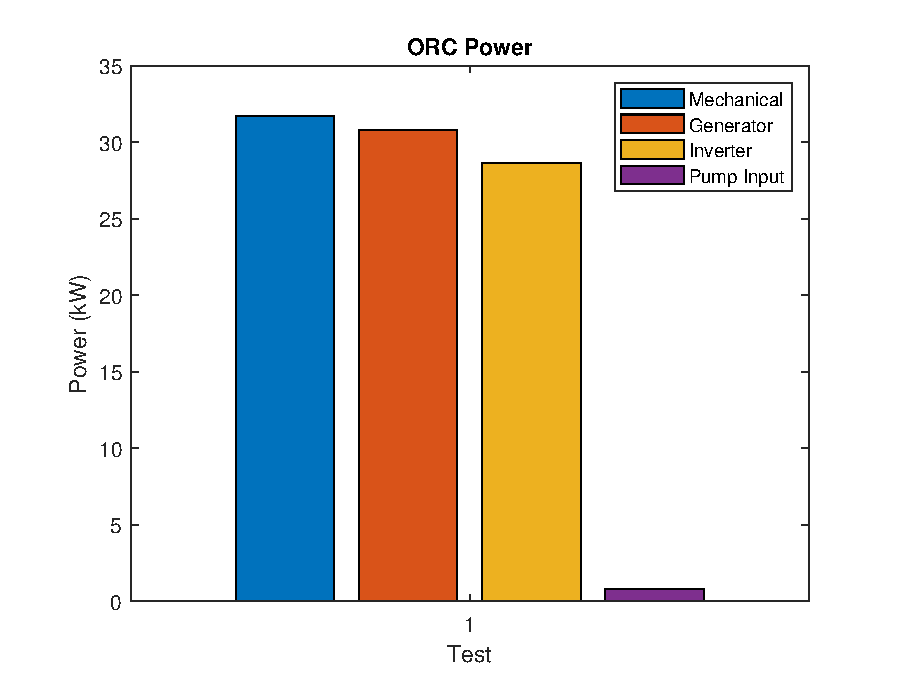
\includegraphics[width=\textwidth]{figures/bfPower}

	\caption{Comparison of mechanical power, generator power, inverter output power, and pump power consumption for the brownfield case of the ORC prime power system model. The test assumes a source temperature of \SI{368}{\kelvin} (\SI{95}{\degreeCelsius}) and a sink temperature of \SI{278}{\kelvin} (\SI{5}{\degreeCelsius}). The source is assumed to flow at a rate of \SI{6}{\liter\per\minute} while the sink flows at \SI{7}{\liter\per\minute}. }
	%Psetpoint[2.75e4;4.0e4;3.08e4;4.2e4;]
	\label{fig:bfPower}
\end{figure}

\autoref{fig:bf_themoplots} shows similar thermodynamic plots as the greenfield scenario. The top right point of each plot represents the state of the working fluid as it is leaving the evaporator before entering the expander. It can be seen that this point lies on the vaporization curve. This means if the working fluid mass flow rate were to increase in order to get more power out, then the fluid would not fully vaporize and the expander efficiency assumption would no longer be valid.
If the amount of heat transferred could be increased, then it's possible the working fluid flow rate could increase as well while maintaining full vaporization. 
\begin{figure}[h]
	\centering

	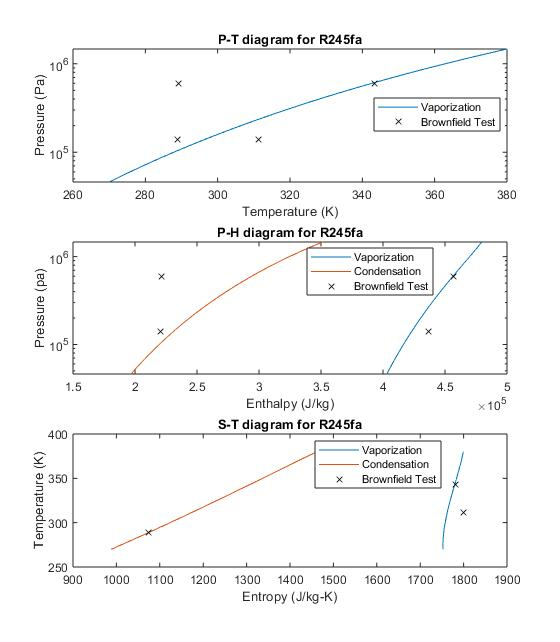
\includegraphics[width=\textwidth]{figures/BrownfieldThermoPlots}
	%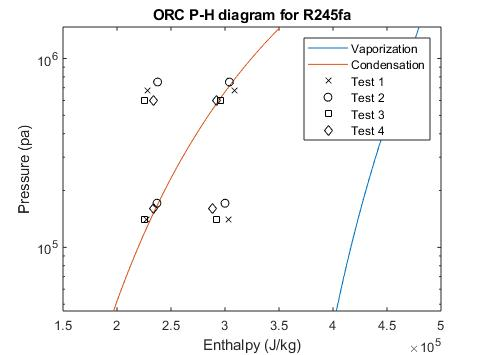
\includegraphics{figures/VerificationPH01}
	\caption{Thermodynamic plots from the simulated brownfield ORC prime power system plotting pressure against temperature (top), pressure against mass specific enthalpy (middle), and temperature against mass specific entropy (bottom). Source temperature and flow rate are assumed to be \SI{368}{\kelvin} (\SI{95}{\degreeCelsius}) and \SI{6}{\liter\per\second}. Sink temperature and flow rate are assumed to be \SI{278}{\kelvin} (\SI{5}{\degreeCelsius}) and \SI{7}{\liter\per\second}.}
	\label{fig:bf_themoplots}
\end{figure}

\cleardoublepage